\newpage 

\section{Polynomial Interpolation}

\emph{Polynomial interpolation} is a family of procedures to find a polynomial given 
a certain numbers of data points \((x_0, y_0), \dots, (x_n, y_n)\) such that 

\[
    f(x_i) = y_i, \quad \forall i = 0, 1, \dots, n.
\]

This results into finding a polynomial with at most degree\(n\), with \(n + 1\) terms and \(n\) constant terms \(c_i\)

\[
    f(x) = c_0 + c_1 x + c_2 x^2 + \dots + c_{n}x^n
\]

\subsection{Set of Polynomials of Degree \texorpdfstring{\(n\)}{n}}

We define the set of polynomials with at degree \(n\) as \(P_n\).

\subsection{Maximal Number of Zeros For A Polynomial}

A polynomial \(p \in P_n\) has at most \(n\) zeros or is identical 0.

\subsection{Uniqueness of The Polynomial Interpolation}

Given a set of points \((x_0, y_0), \dots, (x_n, y_n)\) there exists only one polynomial of degree at most \(n\) 
such that \(f(x_0) = y_0, \dots\).

\textbf{Proof:}

\emph{Uniqueness}: Let us assume that such a polynomial \(p(x)\) exists, and also \(q(x) \ne p(x)\) such that both interpolate our 
points.

Using the fact that a polynomial \(P_n\) has at most \(n\) zeros or is identical 0.

If we perform the following operation

\[
    p(x) - q(x) = 0, \quad \forall x \in \{x \mid (x, y), \ y = 0\}
\]

We have a polynomial \(p(x) - q(x) \in P_n\) but it has zeros at \(n + 1\) places, hence \(p(x) - q(x) = 0 \implies p(x) = q(x)\).

\subsection{Vandermonde Systems}

For our interpolation \(p(x)\) we define the following system 

\[
    Vc 
    =
    \begin{bmatrix}
        1 & x_0 & \dots & x_0^n \\ 
        \vdots & \vdots &  & \vdots \\ 
        1 & x_n & \dots & x_n^n \\ 
    \end{bmatrix}
    \begin{bmatrix}
        c_0 \\ 
        \vdots \\ 
        c_n
    \end{bmatrix}
    = 
    \begin{bmatrix}
        y_0 \\ 
        \vdots \\ 
        y_n
    \end{bmatrix}
    = y
\]

\(Vc = y\) as our \emph{Vandermonde system} with \(V\) as the \emph{Vandermonde matrix}.

Now our problem of finding the constants in the vector \(c\) has been transformed into finding the inverse of \(V\).

\subsubsection{Invertibility Of The Vandermonde Matrix}

There exits an \(V^{-1}\) to the corresponding \(V\).

\textbf{Proof:}

\(\exists V^{-1} \iff \det(V) \ne 0\), therefore we need to compute the determinant in the following way.

Remember that row/column operations do not change the determinant 

\[
    \det(A) = \det(A')  =\det(C_i A) = \det(C_i)\det(A) = 1 \cdot \det(A)
\]

For 

\[
    V = 
    \begin{bmatrix}
        1 & x_0 & x_0^2 & \dots & x_0^n \\ 
        1 & x_1 & x_1^2 & \dots & x_1^n \\ 
        \vdots &  \vdots & \vdots&  & \vdots \\ 
        1 & x_n & x_n^2 & \dots & x_n^n \\ 
    \end{bmatrix}
\]

We add from the first column times \(-x_0\), then the second \(x_0 x_1\) and so on for each column

\begin{align*}
    \det(V) &= \det
    \begin{bmatrix}
        1 & x_0 & x_0^2 & \dots & x_0^n \\ 
        1 & x_1 & x_1^2 & \dots & x_1^n \\ 
        \vdots &  \vdots & \vdots&  & \vdots \\ 
        1 & x_n & x_n^2 & \dots & x_n^n
    \end{bmatrix} \\ 
    &= 
    \det
    \begin{bmatrix}
        1 & 0 & 0 & \dots & 0 \\ 
        1 & x_1 & x_1^2 & \dots & x_1^n \\ 
        \vdots &  \vdots & \vdots&  & \vdots \\ 
        1 & x_n & x_n^2 & \dots & x_n^n
    \end{bmatrix} \\ 
    &= 
    \det
    \begin{bmatrix}
        1 & 0 & 0 & \dots & 0 \\ 
        1 & x_1 - x_0 & x_1^2 -x_0 x_1 & \dots & x_1^n  - x_0x_1^{n - 1}\\ 
        \vdots &  \vdots & \vdots&  & \vdots \\ 
        1 & x_n - x_0 & x_n^2 -x_0 x_n & \dots & x_n^n - x_0 x_n^{n - 1}
    \end{bmatrix} \\ 
    &= 
    \det
    \begin{bmatrix}
        1 & 0 & 0 & \dots & 0 \\ 
        1 & x_1 - x_0 & x_1(x_1^2 -x_0) & \dots & x_1^{n - 1}( x_1 - x_0)\\ 
        \vdots &  \vdots & \vdots&  & \vdots \\ 
        1 & x_n - x_0 &x_n (x_n - x_0) & \dots & x_n^{n - 1}(x_n - x_0)
    \end{bmatrix} \\ 
    &= (x_1 - x_0)(x_2 - x_0) \cdot \dots \cdot (x_n - x_0) \det
    \begin{bmatrix}
        1 & x_1 & \dots & x_1^{n - 1} \\ 
        \vdots & \vdots &  & \vdots \\ 
        1 & x_n & \dots & x_n^{n - 1} 
    \end{bmatrix}
\end{align*}

By repeatedly applying the column subtraction, we get a transformed matrix from which we can extract the scalar factors from each 
column and then using the Laplace method for determinants, repeat the process for the inner sub-matrix.

Giving us an inductive procedure and the following results 

\[
    \det(V) = \prod_{0 \le i < j \le n} (x_j - x_i) \neq 0 \iff x_i \ne x_j \ \forall i \ne j.
\]

\subsection{Lagrange Polynomials}

\emph{Lagrange polynomial} are used to interpolate polynomial by using the following property

\[
    L_j(x_i) = 
    \begin{cases}
       1, & \, i = j \\  
       0, &  
    \end{cases}
\]

This is done by the definition 

\[
    L_j (x) = \prod_{i = 0}^{j - 1} \frac{x - x_i}{x_j- x_i} \prod_{i = 1}^{n} \frac{x - x_{j + i}}{x_j - x_{j + i}} = \prod_{i = 0, i \ne j}^{n} \frac{x - x_i}{x_j - x_i}
\]

This comes from the fact that given our points \(x_0, x_1, \dots x_n\) and we want for \(x_n\) that \(L_m(x_m) = 1\) and zero else where we get 

\[
    (x - x_1)(x - x_2)\cdot \dots \cdot (x - x_{m - 1})(x - x_{m + 1}) \cdot \dots \cdot \dot (x - x_n) \ne 1, \quad \text{but zero for every other}\, x_k
\]

To get it to be 1, we just need to normalize the term

\[
    \frac{(x - x_1)(x - x_2)\cdot \dots \cdot (x - x_{m - 1})(x - x_{m + 1}) \cdot \dots \cdot \dot (x - x_n)}{(x_m - x_1)(x_m - x_2)\cdot \dots \cdot (x_m - x_{m - 1})(x_m - x_{m + 1}) \cdot \dots \cdot \dot (x_m - x_n)}
\]

Our Lagrange polynomial is defined as 

\[
    p(x) = \sum_{i = 0}^{n} y_i L_i(x_i) = \sum_{i = 0}^{n} y_i  \left[\prod_{i = 0, i \ne j}^{n} \frac{x - x_i}{x_j - x_i}\right]
\]

\textbf{Example:}

Given are the points \((0, 3), (1, 2), (3, 6)\) find the interpolating polynomial.

\[
    L_0(x) = \frac{(x - 1)(x - 3)}{(0 - 1)(0 - 3)} = \frac{(x - 1)(x - 3)}{3} 
\]

\[
    L_1(x) = \frac{(x - 0)(x - 3)}{(1 - 0)(1 - 3)} = \frac{(x)(x - 3)}{-2}
\]

\[
    L_2(x) = \frac{(x - 0)(x - 1)}{(3 - 0)(3 - 1)} = \frac{(x)(x - 1)}{6}
\]

Resulting in the following interpolating polynomial

\[
    p(x) = 3 \cdot \frac{(x - 1)(x - 3)}{3} + 2 \cdot \frac{(x)(x - 3)}{-2} + 6 \cdot \frac{(x)(x - 1)}{6} = x^2 - x + 3
\]


\subsection{Newton Polynomials}

The interpolation polynomial in the \emph{Newtonian form} is a defined as 

\[
    p(x) = y_0 + a_1(x - x_0) + a_2(x - x_0)(x - x_1) + \dots + a_n \prod_{i = 0}^{n-1} (x - x_i)
\]

Note, that for for \(p(x) = y_0 + a_1(x - x_0)\) if we put \(p(x_0) = y0\) which is a quality we want.  If we set 
our polynomial to \(y_1\) we also get the first \emph{divided difference} 

\[
    y_1 = y_0 + a_1 (x_1 - x_0) \iff a_1 = \frac{y_1 - y_0}{x_1 - x_0} = f[x_0, x_1]
\]

where \(f[x_i, x_j]\) is the \emph{divided difference} defined as

\[
    f[x_i, x_j] = \frac{f[x_i, j -1] - f[x_{i - 1}, x_{j - 1}]}{x_i - x_{i - j}}
\]

with 

\[
    f[x_i, 0] = y_i
\]


We can keep the step we did without a recurrence relation for the next higher degree polynomials and get all of our differences.

\subsubsection{Recurrence Relation Table}

When working out an exercise, it is useful to write down the divided differences in a table as follows:

\begin{center}
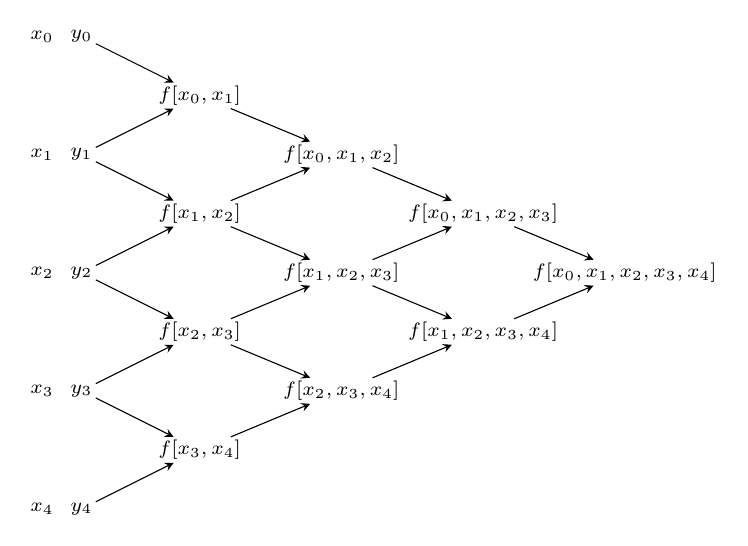
\begin{tikzpicture}[
    ->, >=stealth,
    every node/.style={font=\scriptsize, inner sep=1pt}
]

% Per-column x positions (cm): x | y | 1st | 2nd | 3rd | 4th
\def\cx{0}
\def\cy{0.5}
\def\ca{2.0}
\def\cb{3.8}
\def\cc{5.6}
\def\cd{7.4}
\def\ys{0.75}

% x_i labels
\node at (\cx,       0)    {$x_0$};
\node at (\cx, -2*\ys)     {$x_1$};
\node at (\cx, -4*\ys)     {$x_2$};
\node at (\cx, -6*\ys)     {$x_3$};
\node at (\cx, -8*\ys)     {$x_4$};

% y_i (zeroth divided differences)
\node (y0) at (\cy,       0)   {$y_0$};
\node (y1) at (\cy, -2*\ys)    {$y_1$};
\node (y2) at (\cy, -4*\ys)    {$y_2$};
\node (y3) at (\cy, -6*\ys)    {$y_3$};
\node (y4) at (\cy, -8*\ys)    {$y_4$};

% 1st divided differences
\node (f01) at (\ca, -1*\ys) {$f[x_0,x_1]$};
\node (f12) at (\ca, -3*\ys) {$f[x_1,x_2]$};
\node (f23) at (\ca, -5*\ys) {$f[x_2,x_3]$};
\node (f34) at (\ca, -7*\ys) {$f[x_3,x_4]$};

% 2nd divided differences
\node (f02) at (\cb, -2*\ys) {$f[x_0, x_1, x_2]$};
\node (f13) at (\cb, -4*\ys) {$f[x_1, x_2, x_3]$};
\node (f24) at (\cb, -6*\ys) {$f[x_2, x_3, x_4]$};

% 3rd divided differences
\node (f03) at (\cc, -3*\ys) {$f[x_0,x_1, x_2, x_3]$};
\node (f14) at (\cc, -5*\ys) {$f[x_1, x_2, x_3, x_4]$};

% 4th divided difference
\node (f04) at (\cd, -4*\ys) {$f[x_0, x_1, x_2, x_3, x_4]$};

% y_i -> 1st differences
\draw (y0) -- (f01);
\draw (y1) -- (f01);
\draw (y1) -- (f12);
\draw (y2) -- (f12);
\draw (y2) -- (f23);
\draw (y3) -- (f23);
\draw (y3) -- (f34);
\draw (y4) -- (f34);

% 1st -> 2nd differences
\draw (f01) -- (f02);
\draw (f12) -- (f02);
\draw (f12) -- (f13);
\draw (f23) -- (f13);
\draw (f23) -- (f24);
\draw (f34) -- (f24);

% 2nd -> 3rd differences
\draw (f02) -- (f03);
\draw (f13) -- (f03);
\draw (f13) -- (f14);
\draw (f24) -- (f14);

% 3rd -> 4th difference
\draw (f03) -- (f04);
\draw (f14) -- (f04);

\end{tikzpicture}
\end{center}

Although the table looks complicated, when using the actual values for \(x_i\) and \(x_j\) we follow a simple pattern to fill in the table of 
going up the diagonally down and up, starting. For example for 

\[
    f[x_0, x_1] = \frac{y_1 \text{ (start) } - y_0 \text{ (up)}}{x_1 \text{ (diagonally down) } - x_0 \text{ (up) }}
\]

It is important to note that the first column of the table is just the \(y_i\) values, for the next columns we use the previous column to compute nominator and the denominator is 
still defined by the \(x_i\) values.

\textbf{Example:}

Given are the points \((0, 3), (1, 2), (3, 6)\) find the interpolating polynomial.

We start by filling in the first column of the table with the \(y_i\) values

\medskip

\begin{center}
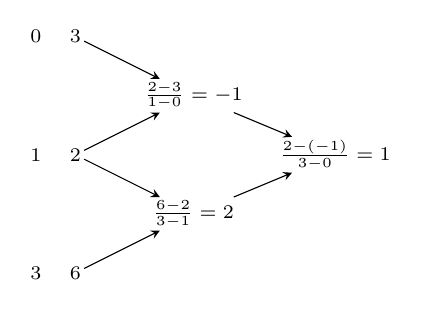
\begin{tikzpicture}[
    ->, >=stealth,
    every node/.style={font=\scriptsize, inner sep=1pt}
]

\def\cx{0}
\def\cy{0.5}
\def\ca{2.0}
\def\cb{3.8}
\def\ys{0.75}

% x_i labels
\node at (\cx,       0)    {$0$};
\node at (\cx, -2*\ys)     {$1$};
\node at (\cx, -4*\ys)     {$3$};

% y_i (zeroth divided differences)
\node (y0) at (\cy,       0)   {$3$};
\node (y1) at (\cy, -2*\ys)    {$2$};
\node (y2) at (\cy, -4*\ys)    {$6$};

% 1st divided differences
\node (f01) at (\ca, -1*\ys) {$\frac{2 - 3}{1 - 0} = -1$};
\node (f12) at (\ca, -3*\ys) {$\frac{6 - 2}{3 - 1} = 2$};

% 2nd divided differences
\node (f02) at (\cb, -2*\ys) {$\frac{2 - (-1)}{3 - 0} = 1$};

% y_i -> 1st differences
\draw (y0) -- (f01);
\draw (y1) -- (f01);
\draw (y1) -- (f12);
\draw (y2) -- (f12);

% 1st -> 2nd differences
\draw (f01) -- (f02);
\draw (f12) -- (f02);

\end{tikzpicture}
\end{center}

The resulting interpolating polynomial is

\[
    p(x) = 3 + (-1)(x - 0) + 1(x - 0)(x - 1) = x^2 - x + 3
\]